%%%%%%%%%%%%%%%%%%%%%%%%%%%%%%%%%%%%%%%%%
% Simple Sectioned Essay Template
% LaTeX Template
%
% This template has been downloaded from:
% http://www.latextemplates.com
%
% Note:
% The \lipsum[#] commands throughout this template generate dummy text
% to fill the template out. These commands should all be removed when
% writing essay content.
%
%%%%%%%%%%%%%%%%%%%%%%%%%%%%%%%%%%%%%%%%%

%----------------------------------------------------------------------------------------
%	PACKAGES AND OTHER DOCUMENT CONFIGURATIONS
%----------------------------------------------------------------------------------------

\documentclass[12pt]{article} % Default font size is 12pt, it can be changed here

\usepackage{geometry} % Required to change the page size to A4
\geometry{a4paper} % Set the page size to be A4 as opposed to the default US Letter

\usepackage{graphicx} % Required for including pictures

\usepackage{float} % Allows putting an [H] in \begin{figure} to specify the exact location of the figure
\usepackage{wrapfig} % Allows in-line images such as the example fish picture

\usepackage{lipsum} % Used for inserting dummy 'Lorem ipsum' text into the template

\usepackage{multicol}
\usepackage{amsmath}

\usepackage[utf8x]{inputenc}
\usepackage{amsfonts,euscript,latexsym,amssymb}
\usepackage[portuguese,USenglish]{babel}

\linespread{1.2} % Line spacing

%\setlength\parindent{0pt} % Uncomment to remove all indentation from paragraphs

\graphicspath{{Pictures/}} % Specifies the directory where pictures are stored

\begin{document}

%----------------------------------------------------------------------------------------
%	TITLE PAGE
%----------------------------------------------------------------------------------------

\begin{titlepage}

\newcommand{\HRule}{\rule{\linewidth}{0.5mm}} % Defines a new command for the horizontal lines, change thickness here

\center % Center everything on the page

\textsc{\LARGE Instituto Superior Tecnico}\\[1cm] % Name of your university/college
\textsc{\Large Programação de Sistemas}\\[0.5cm] % Major heading such as course name
\textsc{\large}\\[0.5cm] % Minor heading such as course title
\HRule \\[0.4cm]
{ \LARGE \bfseries Key-Value Store}\\[0.4cm]
% Title of your document
\HRule \\[1cm]

\begin{minipage}{0.6\textwidth}
\begin{flushleft} \large
\emph{Autores:}\\
73640 - André \textsc{Stielau}\\
73198 - João \textsc{Almeida}\\

\end{flushleft}
\end{minipage}
~
\\[1cm]
{\large 29 de Maio de 2016}\\[1cm] % Date, change the \today to a set date if you want to be precise

\begin{figure}[H]
\centering

\includegraphics[width=0.7\textwidth]{./Pictures/tecnico.png}
\end{figure}

\vfill % Fill the rest of the page with whitespace

\end{titlepage}

%----------------------------------------------------------------------------------------
%	TABLE OF CONTENTS
%----------------------------------------------------------------------------------------

%\tableofcontents % Include a table of contents

%\newpage % Begins the essay on a new page instead of on the same page as the table of contents

%----------------------------------------------------------------------------------------
%	INTRODUCTION
%----------------------------------------------------------------------------------------

\iffalse

O relatório deverá conter a seguinte informação

Esquema dos componentes e suas ligações
Detalhes de implementação de cada um dos componentes
Detalhes dos modelos de comunicação entre componentes (funcionalidade e protocolos)

Na descrição dos componentes é necessário referir explicitamente o seguinte

Estrutura de dados que armazena os pares (chave, valor)
Mecanismos de sincronização no acesso à estrutura de dados
Mecanismo de gestão da Threads
Protocolo de tolerância à falta
Protocolo de backup/recuperação dos dados
Tratamento de erros
\fi

\section{System overview}
\label{sec:Systemoverview}

To use the Key-Value Store the client uses the \emph{psiskv.h} library to establish a connection and make requests.

The communication flow is exemplified on figure~\ref{fig:Comms}. During the \textbf{kv\_connect} the \textbf{client} connects to the \textbf{Front Server} which responds with the port of the \textbf{Data Server} and then the client connects to it and is ready to make requests.

\begin{figure}[H]
\centering
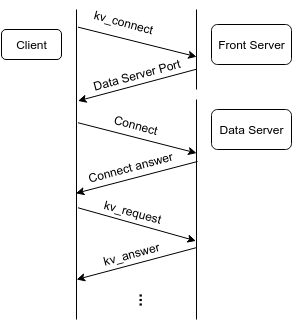
\includegraphics[width=0.6\textwidth]{./Pictures/CommunicationFlow.png}
\caption{Overview of the client KV store communication flow}\label{fig:Comms}
\end{figure}
\section{Key Value Data Structure}

The \textbf{data storage} is implemented on an \textbf{hash table} where each bucket of the hash table is a \textbf{linked list} and each list entry holds the key and a pointer to the value. See Figure~\ref{fig:DataOverview} for more details.

\begin{figure}[H]
\centering
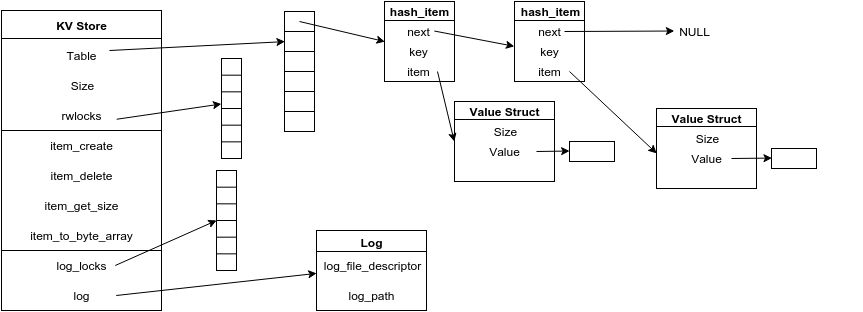
\includegraphics[width=\textwidth]{./Pictures/DataStructures.png}
\caption{Overview of Data Structures}\label{fig:DataOverview}
\end{figure}

The hash table component is implemented with \textbf{data abstraction} in mind, in this system it holds a byte array and its size, but could be used to store any kind of data. The value implementation belongs to other component, in the key-value store case to the \emph{psiskv\_server.h}.

\section{KV Message Formats}

The structure of the messages exchanged between the \textbf{client} and the \textbf{Data server} is:  a  enumerate \emph{msg\_type}, a \emph{uint32\_t} with the \textbf{key} and an \emph{unsigned int} with the length of the value. The possible message types are:
\begin{description}
    \item[WRITE\_REQ] - write request;
    \item[WRITE\_REQ\_OW] - write request with overwrite;
    \item[WRITE\_RESP] - write response;
    \item[READ\_REQ] - read request;
    \item[READ\_RESP] - read response;
    \item[DELETE\_REQ] - delete request;
    \item[DELETE\_RESP] - delete response;
    \item[ERROR] - error message;
\end{description}
After a \emph{WRITE\_REQ} or a \emph{READ\_RESP} a buffer containing the value to store is transmitted over TCP with the length being specified on the previous message.

\subsection{Error Messages}
\label{sub:ErrorMessages}


\section{Data Server}
\label{sec:DataServer}

\subsection{Thread Management}
\label{sub:ThreadManagement}

The threads are created following the \textbf{on demand} strategy.

\section{Front Server}
\label{sec:FrontServer}

\section{Backup and Log}
\label{sec:BackupLog}

To guarantee data consistency a backup and a log file are used.

\section{Fault Tolerance}
\label{sec:FaultTolerance}

\section{Clients}
\label{sec:Clients}








\end{document}
